\begin{figure}[!h]
\centering
\begin{subfigure}[b]{0.5\textwidth}
\centering
	%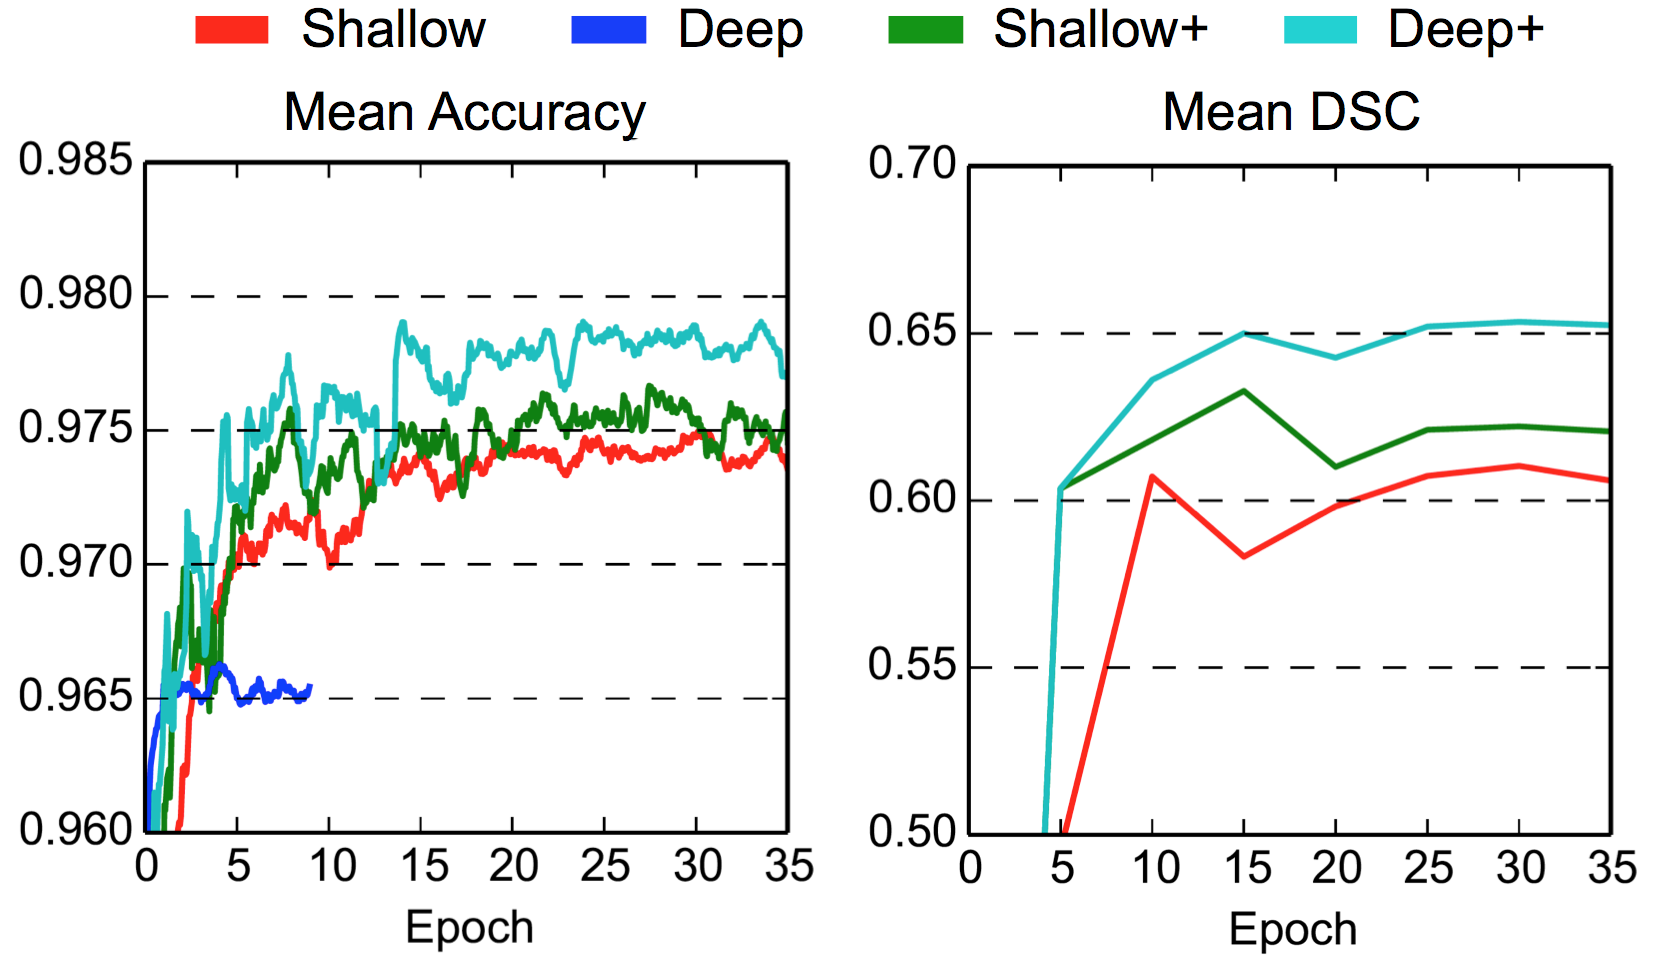
\includegraphics[clip=true, trim=50pt 30pt 140pt 250pt, width=1.0\textwidth]{figures/validationOfArchitecture/deepProblems/deepFigureToPut.pdf}
	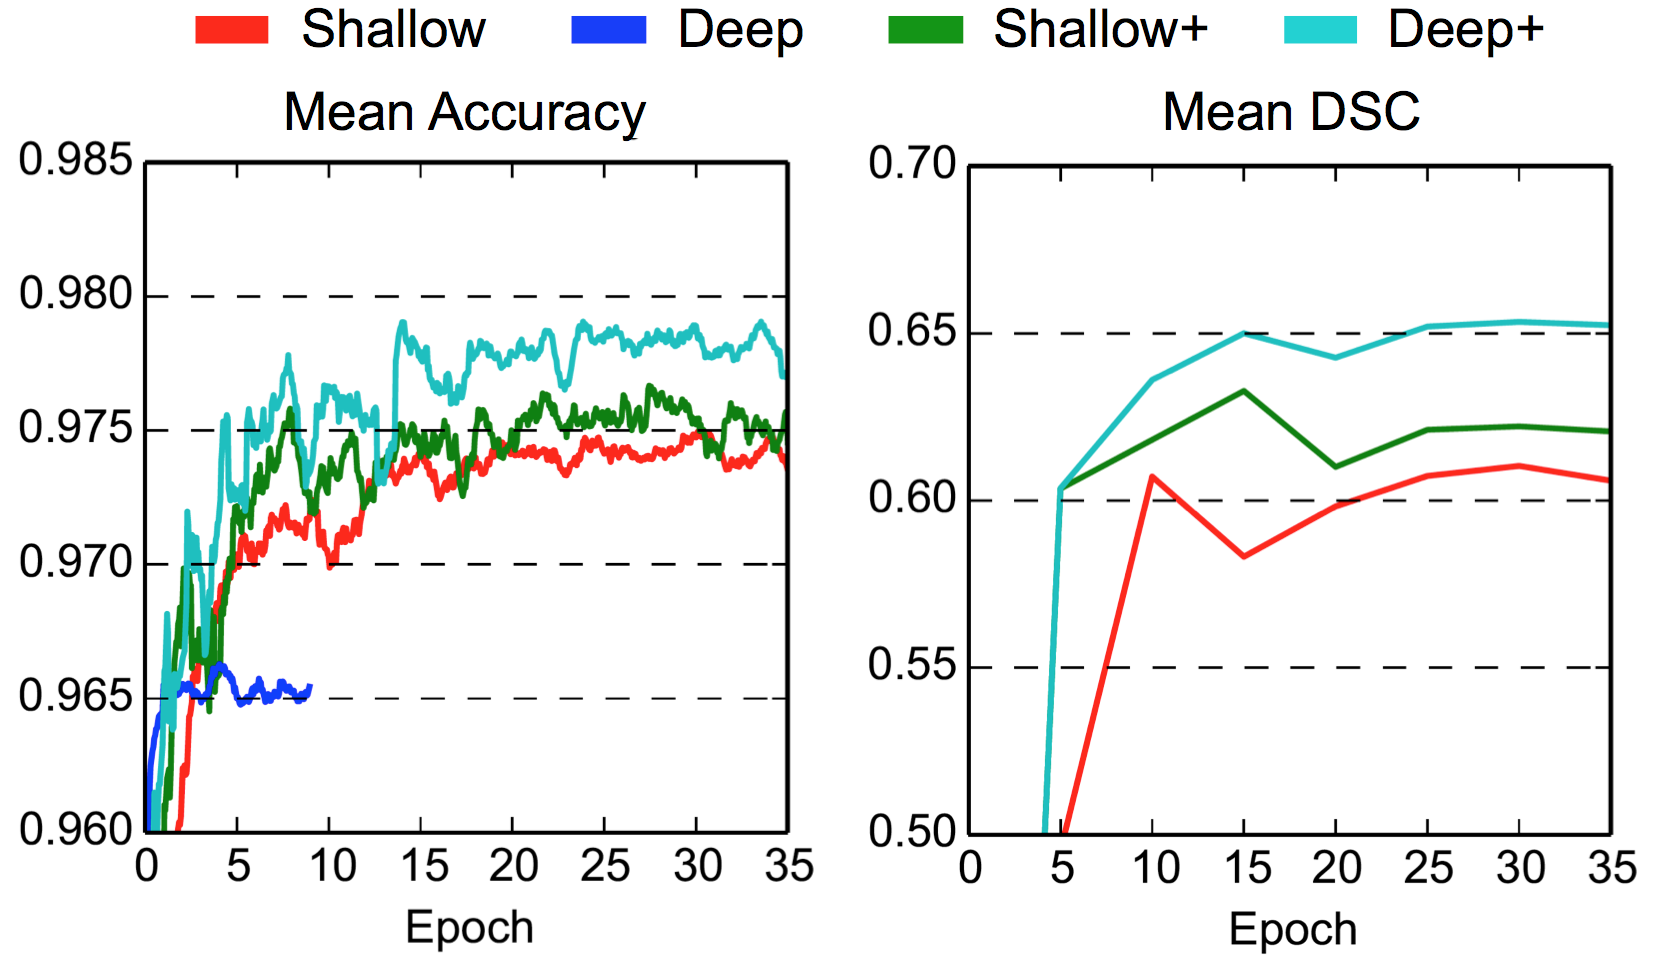
\includegraphics[clip=true, trim=0pt 0pt 0pt 0pt, width=1.0\textwidth]{figures/validationOfArchitecture/deepProblems/deepFigureToPut.png}
\end{subfigure}
\caption{Mean accuracy over validation samples and DSC for the segmentations of the validation images, as obtained from the \quot{Shallow} baseline and \quot{Deep} variant with smaller kernels. Training of the plain deeper model fails (cf. Sec.~\ref{subsec:valDeeper}). This is overcome by adopting the initialization scheme of (\cite{he2015delving}), which further combined with Batch Normalization leads to the enhanced (\texttt{+}) variants. Deep\texttt{+} performs significantly better than Shallow\texttt{+} with similar computation time, thanks to the use of small kernels.
}
\label{fig:deepProblems}
\end{figure}
%\vspace{-1pt} %takes away some white space before figure